\chapter{Introduction}

We live in an era marked by the confluence of environmental challenges and technological innovation. The rapid pace of global change poses a significant and ever-present threat to human well-being. To accelerate the development of new remediation and mitigation strategies we must make \textit{data-driven decisions}. Yet, the constraints imposed by the lack of widely accessible, fine-resolution data, in conjunction with the formidable computational complexities intrinsic to large-scale physics simulations, markedly limits our capacity to develop the accurate assessments needed to address these pressing issues in a timely and substantive manner. By leveraging the data driven techniques of machine learning, we can bridge the data-model gap to transform the data we do have into the quantities we need to produce actionable environmental insights.

\section{Motivation: Global Change and the Need for Improved Sensing Capabilities}

Global change encompasses significant and long-term alterations in the Earth's physical, chemical, and biological systems, arising from both natural processes and human activities \cite{IPCC2014, IPCC2018, UN2015}. These alterations include changes in climate, land use, biodiversity, and biogeochemical cycles, as well as the intricate interactions among these systems. Global change exerts profound impacts on both natural and human systems, manifesting as shifts in weather patterns, rising sea levels, heightened frequency and severity of extreme events, loss of biodiversity and ecosystem services, and adverse effects on human health and well-being. The comprehension and effective management of global change present critical challenges for society today, necessitating interdisciplinary approaches and international collaboration. Comprehensive environmental sensing plays a pivotal role by providing real-time data across these crucial areas, aiding in the identification and resolution of environmental concerns.

Global change can profoundly impact human health, both through direct and indirect mechanisms. For instance, the rise in global temperatures escalates the susceptibility to heat-related ailments like heat exhaustion and heat stroke. This heightened risk is particularly concerning for vulnerable demographics, including the elderly, young children, and outdoor workers \cite{WHO2018, Costello2009, Haines2006}. Furthermore, exposure to air pollution is associated with an increased likelihood of developing respiratory and cardiovascular diseases, such as asthma, chronic obstructive pulmonary disease (COPD), and heart disease. Shifts in temperature and precipitation patterns can influence the distribution and abundance of disease vectors like mosquitoes and ticks, thereby elevating the threat of vector-borne diseases, including dengue fever, malaria, and Lyme disease. In a similar vein, alterations in precipitation patterns and water quality can heighten the risk of waterborne diseases, notably cholera. Food availability and production can also be impacted, potentially resulting in food shortages and malnutrition, among vulnerable populations.


\subsection{Air Quality}

\begin{table}[h!]
  \centering
  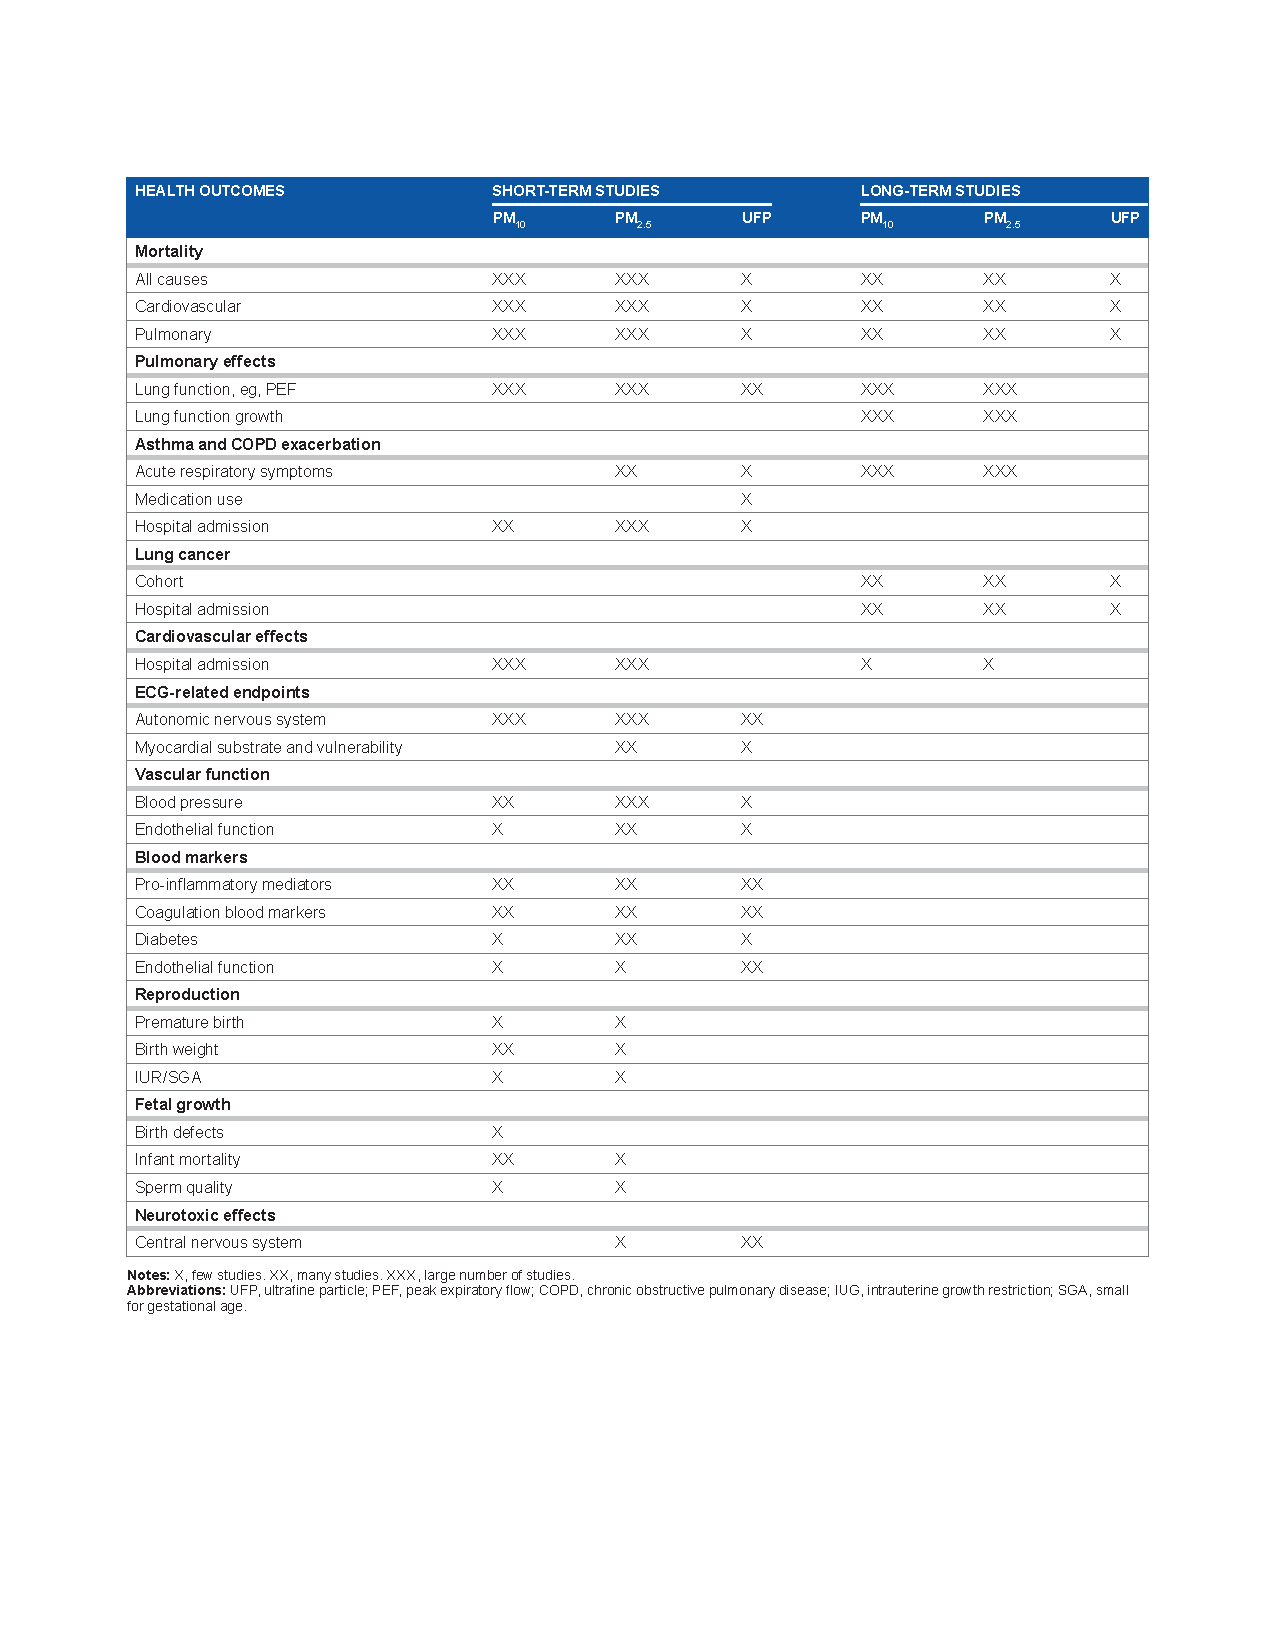
\includegraphics[width=\textwidth]{introduction/HealthEffectsParticulates.pdf}
	\caption{Tabular literature review of particulate matter and health outcomes related to PM$_{10}$, PM$_{2.5}$, and ultrafine particulates (UFPs) exposure (based on the literature review of \cite{Lary:2015}).}
	\label{Table.HealthEffectsParticulates}
\end{table}


Taking air quality as a particularly poignant example, the World Health Organization (WHO) estimates that over 90\% of the world's population breathes air that exceeds air quality guidelines for fine particulate matter (PM2.5) concentrations \cite{world2021global}. Ambient air pollution is estimated to cause 4.2 million premature deaths worldwide each year. In comparison, the total number of global confirmed COVID-19 deaths in 2020 was 1.9 million, and 3.6 million in 2021. Even at the height of the COVID pandemic, deaths from poor air quality outnumbered those from COVID-19. The quality of outdoor ambient air, in turn, influences the quality of indoor air. In areas where outdoor air quality is already poor, increasing ventilation inevitably introduces pollutants indoors, even when filtration is employed \cite{srikrishna_long-term_2022}. While death is unquestionably the most severe consequence of pollution, it is far from the only one. The biological wear and tear caused by poor air quality has been shown to degrade cognitive and physical performance, as well as a variety of human health outcomes \cite{Krebs2021AirPC, Gao2021ShorttermAP, Carneiro2021TheEO, Ni2021AssociationsOP, Shehab2019EffectsOS} like those listed in Table \ref{Table.HealthEffectsParticulates}. Degraded cognitive performance has a significant impact on society, ranging from poor learning outcomes in schools to impaired decision-making and productivity at work. As a result, the ability to adequately and comprehensively quantify the key markers of air quality is critical for guiding appropriate, science-based mitigation strategies.

\subsection{Air Quality Indoors}

Humans spend approximately 90\% of their time indoors \cite{finewax_quantification_2021}. Consequently, the quality of indoor air has a dramatic effect on physical health, cognitive performance, and general well-being \cite{Krebs2021AirPC, Gao2021ShorttermAP, Carneiro2021TheEO, Ni2021AssociationsOP, Shehab2019EffectsOS}. Heating, ventilation, and air conditioning (HVAC) systems are typically designed to circulate air throughout a building, bringing in outside air, in order to achieve comfortable thermal conditions while consuming as little energy as possible \cite{memarzadeh_role_2012}. When assigned the secondary task of maintaining indoor air quality, ventilation operates by the same principles as a laboratory fume hood: airtightness and controlled airflow. To be effective, the ventilation system must move air along a short, unimpeded path toward the exhaust point while preventing unintended leakage \cite{ng_iaq_2015}. Despite these assumptions, most buildings are not airtight nor are they well-mixed \cite{emmerich_investigation_2005}. Further, the variable nature of indoor human interactions coupled with the plethora of possible room configurations introduces significant design challenges. Computational fluid dynamics (CFD) simulations of the airflow in hospital rooms found that ``the most important contributing factor to contaminant transmission in enclosed and mechanically ventilated environment is the path between the contaminant source and the exhaust, not the air changes per hour" \cite{memarzadeh_role_2012}. This observation is widely confirmed across the literature with multiple studies indicating that air changes per hour (ACH) can be safely lowered without increasing concentrations of chemicals of concern above tolerable levels \cite{ng_iaq_2015, lamping_air_nodate, li_evaluation_2014}. In concert with these findings, studies of the transmission of airborne pathogens suggest that increasing the air change rate removes contaminants from the source room faster but also increases the rate of exposure in connected rooms.

Buildings contain significant sources of volatile chemical products such as cleaners, disinfectants, personal care products (PCPs), and paints whose use introduces a variety of potentially harmful compounds into the indoor environment \cite{finewax_quantification_2021}. The growing body of pandemic case studies calls into question the long-held belief that increasing ventilation is the only and best way to control indoor pollution and reduce the spread of airborne pathogens \cite{ng_iaq_2015, zaatari_impact_2016, pease_investigation_2021, zheng_covid-19_2021}. Furthermore, such proposals to focus on increased ventilation rates can only be realized through significant construction and renovation, and once completed, have a significant increase in running costs due to the energy required, preventing our most vulnerable communities from accessing clean air disproportionately \cite{lamping_air_nodate}.

The COVID-19 pandemic has unequivocally demonstrated the need for improved testing and evaluation methodology that characterizes the various components of indoor air quality holistically. This is necessary for the critical evaluation and assessment of built-environment ventilation, filtration, and air-cleaning approaches. Furthermore, given the dual challenges of global pandemics and global change, the carbon footprint of various indoor air quality remediation strategies must be evaluated in order to optimize both indoor air quality and the carbon footprint. If we fail to consider both aspects, we risk inadvertently promoting an increase in health and economic disparities by failing to consider the very real costs associated with increased air changes. Without a doubt, the composition of the ambient environment has a significant impact on human health as well as general human physical and cognitive performance. Even after a significant initial indoor exposure event may have passed, the health impact associated with prior significant and persistent exposure events may well contribute to long-term health quality. For example, chemical disinfectants such as hypochlorite bleach, have been linked to respiratory ailments and have been observed to produce harmful byproducts such as chloroform, carbon tetrachloride, and N-chloroaldimines, which can take up to 3 hours to be ventilated away after the use the bleach  \cite{finewax_quantification_2021, odabasi_halogenated_2008}.

If HVAC control is driven by an incomplete subset of metrics/contaminants of concern, buildings will clearly fail to adapt to unexpected threats. For instance, CO$_2$ is frequently used as a control metric for ventilation because it closely tracks with the number of people in a room. Five studies found that CO$_2$ control alone cannot control for pollutants generated outdoors or indoors independent of human activity \cite{zaatari_impact_2016}. More recently, one COVID-19 case study discovered that the rapid spread of the disease through a nursing home ward was most likely caused by decreased ventilation by a CO$_2$ demand control ventilation system optimized solely for decreased energy-demand \cite{lamping_air_nodate}. Taken together, the consequences of poor air quality coupled with the lack of real time monitoring of key constituents demonstrates the need for an improved understanding of indoor air.


\section{Physics Based Machine Learning}


In recent years machine learning has exploded in popularity becoming entwined in almost every aspect of our lives from image recognition on social media sites, to the now ubiquitous large large language models like ChatGPT. Because the field is so wide, many of the most popular machine learning models must be generic enough so as to apply to \textit{any} well defined regression or classification task. For example, the problem of image classification is incredibly challenging if we do not impose any restrictions on the type of content represented in our data, as illustrated in Figure \ref{fig:dog-or-muffin}.
\begin{figure}[!hbt]
  \centering
  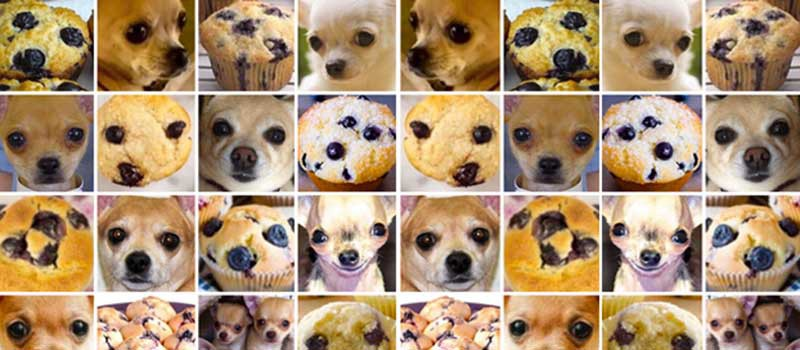
\includegraphics[width=0.6\columnwidth]{introduction/dog-or-muffin.jpeg}
  \caption{A classic machine learning meme comparing pictures of Chihuahuas with muffins illustrating the potential difficulties faced by generic image classification tasks.}
  \label{fig:dog-or-muffin}
\end{figure}
As a consequence, we typically can not expect a machine learning model to generalize beyond the bounds of their training data.

In the realm of scientific applications, this is often \textit{not} the case; the universe is well described by deep physical principles with underlying mathematical symmetries and structures. Therefore, rather than throwing away all of our prior scientific knowledge for each machine learning task, we can instead develop techniques which enable us to directly or indirectly impose physical requirements on our machine learning models. Similarly, we can utilize machine learning to gain insight into physical processes where a first principles relationship has not yet been established. Together these ideas are known as \textit{Physics-Based Machine Learning} or more generally \textit{Scientific Machine Learning} (SciML for short) and provides us the exact set of tools needed to marry scientific models together with data to produce actionable insights \cite{rackauckas2020universal}.


\section{Dissertation Goals}
The goal of this dissertation is to advance physical sensing in service of society by demonstrating the use of new techniques from physics-based machine learning on a variety of real world data sets. Towards this end, this work presents a collection of case studies utilizing both supervised and unsupervised machine learning techniques in a variety of contexts together with physical sensing to produce actionable environmental insights. The applications of this research apply widely across many scientific domains including remote sensing, time series analysis, air quality, chemical kinetics, and data assimilation.

\section{Dissertation Overview}

In chapter 2 we present the relevant sensing techniques employed in each of the three case studies: The first is a autonomous robot team designed to enable the direct estimation of concentrations of chemicals-of-concern in water utilizing an autonomous drone equipped with a hyperspectral imager. The second is a distributed network of low-cost air quality monitors designed to continuously measure key air quality criterion such as particulate matter (PM) and relevant meteorological variables (temperature, pressure, humidity, etc.). The third is a highly advanced measurement chamber designed to evaluate the chemical kinetics of indoor air.

In chapter 3 we present the relevant machine learning background for this work. We also describe open source implementations of Gaussian Process Regression, Self Organizing Maps, and Generative Topographic Mappings, which we developed for use in this dissertation. Machine learning uncertainty quantification methods are discussed including the technique of Conformal Prediction which we now use for all of our supervised regression tasks. Finally, we provide an in depth discussion of data assimilation including both 4D-variational (4d-Var) data assimilation and extended Kalman Filtering (EKF) techniques which we utilize in modeling the chemical reaction kinetics of indoor air.

In chapter 4 we present results for the Robotic Team which consist of three main contributions. The first is the development of an original processing and georectification code which enables the \textit{real time} generation of accurately georectified reflectance datacubes in the field. In the second case study, we demonstrate the use of this robotic team to produce machine learning models mapping reflectance spectra directly to chemical concentrations in a North Texas lake. Finally, we present results of applying our unsupervised learning strategies, namely the SOM and GTM, to deduce the spectral signatures of key chemical constituents without the need for a predetermined spectral data-base.

In chapter 5 we present time series techniques designed for use with our low cost sensing network. The first is a method for using temporal variograms (a statistical technique) to generate reasonable estimates for the intrinsic uncertainty of low cost sensors. The second is an extension of the Hankel Alternative View Of Koopman (HAVOK) method to enable physics-based modeling of our gathered time series. Finally, I train a Hamiltonian Neural Network with a generalized coordinate autoencoder to learn representations of generalized position and momenta for a time series embedding of particulate matter concentrations together with an associated Hamiltonian. Together, the augmented HAVOK model and HNN provide interesting ways to identify transient pollution events from time series.

In chapter 6 we present a novel chemical data assimilation framework for the assessment of indoor air quality. The first major component involves performing a detailed characterization of indoor photolysis using GPR to generate relevant cross section and quantum yield fits from data scraped from a variety of databases. Next we use this photolysis data together with our advanced air quality measurement chamber to evaluate the chemical kinetics of indoor air. Using a combination of 4d-var and the EKF together with a detailed chemical reaction mechanism, we are able to infer the concentrations of reactive species that otherwise well below detectable limits.
%% \section{Completed Work}

%% \subsection{An Autonomous Robotic Team}
%% \subsection{A Distributed Network of Low-Cost Air Quality Monitors}

%% \section{Proposed Work}

%% \subsection{Robot Team}
%% \subsection{Air Quality Network}
%% \subsection{HEART Chamber}
